% Make nice A4 pages for print:
%\usepackage{pgfpages}
%\pgfpagesuselayout{resize to}[a4paper,border shrink=5mm,landscape]

\beamertemplatenavigationsymbolsempty

\setbeamertemplate{bibliography item}[text]

\usepackage[type={CC},modifier={by-sa},version={4.0}]{doclicense}

\usepackage[utf8]{inputenc}
\usepackage{hyperref}
\usepackage{breakurl}
\usepackage{graphicx}
\usepackage{pgfplots}
\usepackage{pgf}
\usepackage{tikz}
\usetikzlibrary{positioning}
\usetikzlibrary{arrows}
\usetikzlibrary{decorations.markings}
\usetikzlibrary{calc}
\usetikzlibrary{matrix}
\usetikzlibrary{shapes}
\usetikzlibrary{decorations.pathmorphing}
\usetikzlibrary{fit}
\usetikzlibrary{backgrounds}
\usetikzlibrary{plotmarks}
\usepackage{stmaryrd}
\usepackage{listings}
\usepackage{pdflscape}
\usepackage{perpage}
\usepackage{appendixnumberbeamer}

%\usepackage[thmmarks,amsmath,amsthm]{ntheorem} % already included in beamer
\usepackage{thm-restate}

\usepackage[sort&compress,numbers]{natbib}  % to be have \citet, \citeauthor, \citeyear

\MakePerPage{footnote}

\tikzstyle{o}=[r,ppBlue]
\tikzstyle{r}=[thick,rectangle,align=center]
\tikzstyle{t}=[r,ppTrans] %,font=\bfseries]
\tikzstyle{dd}=[densely dashed]
\tikzstyle{n}=[r,ppBlue]
\tikzstyle{p}=[r,ppRed]
\tikzstyle{ppRed}  =[draw=red,  fill=  red!20]
\tikzstyle{ppBlue} =[draw=blue, fill= blue!20]
\tikzstyle{ppGreen}=[draw=green,fill=green!20]
\tikzstyle{ppTrans}=[draw=none, fill=none]

\usetheme{Warsaw}

\useoutertheme[subsection=true]{smoothbars}
%\useoutertheme[subsection=false]{miniframes}

\definecolor{bblue}{HTML}{D7DF01}	% yellow-ish actually, for better black/white printing
\definecolor{rred}{HTML}{C0504D}
\definecolor{ggreen}{HTML}{9BBB59}
\definecolor{ppurple}{HTML}{9F4C7C}
\definecolor{lightgray}{rgb}{0.3,0.3,0.3}
\definecolor{lightergray}{rgb}{0.9,0.9,0.9}
\definecolor{UniBlue}{RGB}{83,121,170}

\DeclareTextFontCommand\textintro{\normalfont\bfseries\itshape} % nice!
\newcommand{\intro}[2][]
{%
	\textintro{#2}%
}
\newcommand{\empha}[2][]
{%
	\emph{#2}%
}

%\theoremstyle{plain}
\newcounter{reqcounter}
\newtheorem{requirement}[reqcounter]{Requirement}

%setbeamercolor{structure}{fg=violet}

\makeatletter
\def\th@task{%
    \normalfont % body font
    \setbeamercolor{block title example}{bg=orange,fg=white}
    \setbeamercolor{block body example}{bg=orange!20,fg=black}
    \def\inserttheoremblockenv{exampleblock}
  }
\makeatother

\theoremstyle{task}
\newtheorem{task}{Task}

\newenvironment{assignment}%
{%\setbeamercolor{background canvas}{bg=violet}%
%\setbeamercolor{structure}{fg=cyan!90!black}%
 \setbeamercolor{frametitle}{bg=orange,fg=white}
\begin{frame}}%
{\end{frame}}%

\AtBeginSection[]{
  \begin{frame}
  \vfill
  \centering
  \begin{beamercolorbox}[sep=8pt,center,shadow=true,rounded=true]{title}
    \usebeamerfont{title}\insertsectionhead\par%
  \end{beamercolorbox}
  \tableofcontents
  \vfill
  \end{frame}
}




\pgfplotsset{compat=1.14}
\author{Markus Raab}


\title{LRE Recapitulation}
\date{23.06.2021}

\begin{document}


%%%%%%%%%%%%%%%%%%%%%%%%%%%%%%%%%%%%%%%%%% 
\section{Recapitulation}

\subsection{}

\begin{frame}
	\frametitle{Configuration File Formats (Recapitulation)}
	\methodQuestion{} \question{In which way have you used or contributed to the configuration system/library/API in your previously mentioned FLOSS project(s)?}~\cite{raab2017challenges}
	\pause
	\begin{itemize}
	\item \p{19} persons ($n=251$) have introduced a configuration file format.
	\item \p{29} implemented a configuration file parser.
	\item \p{15} introduced a configuration system/library/API.
	\item \p{34} used external configuration access APIs.
	\end{itemize}
\end{frame}

\begin{frame}
	\frametitle{Current Situation}
	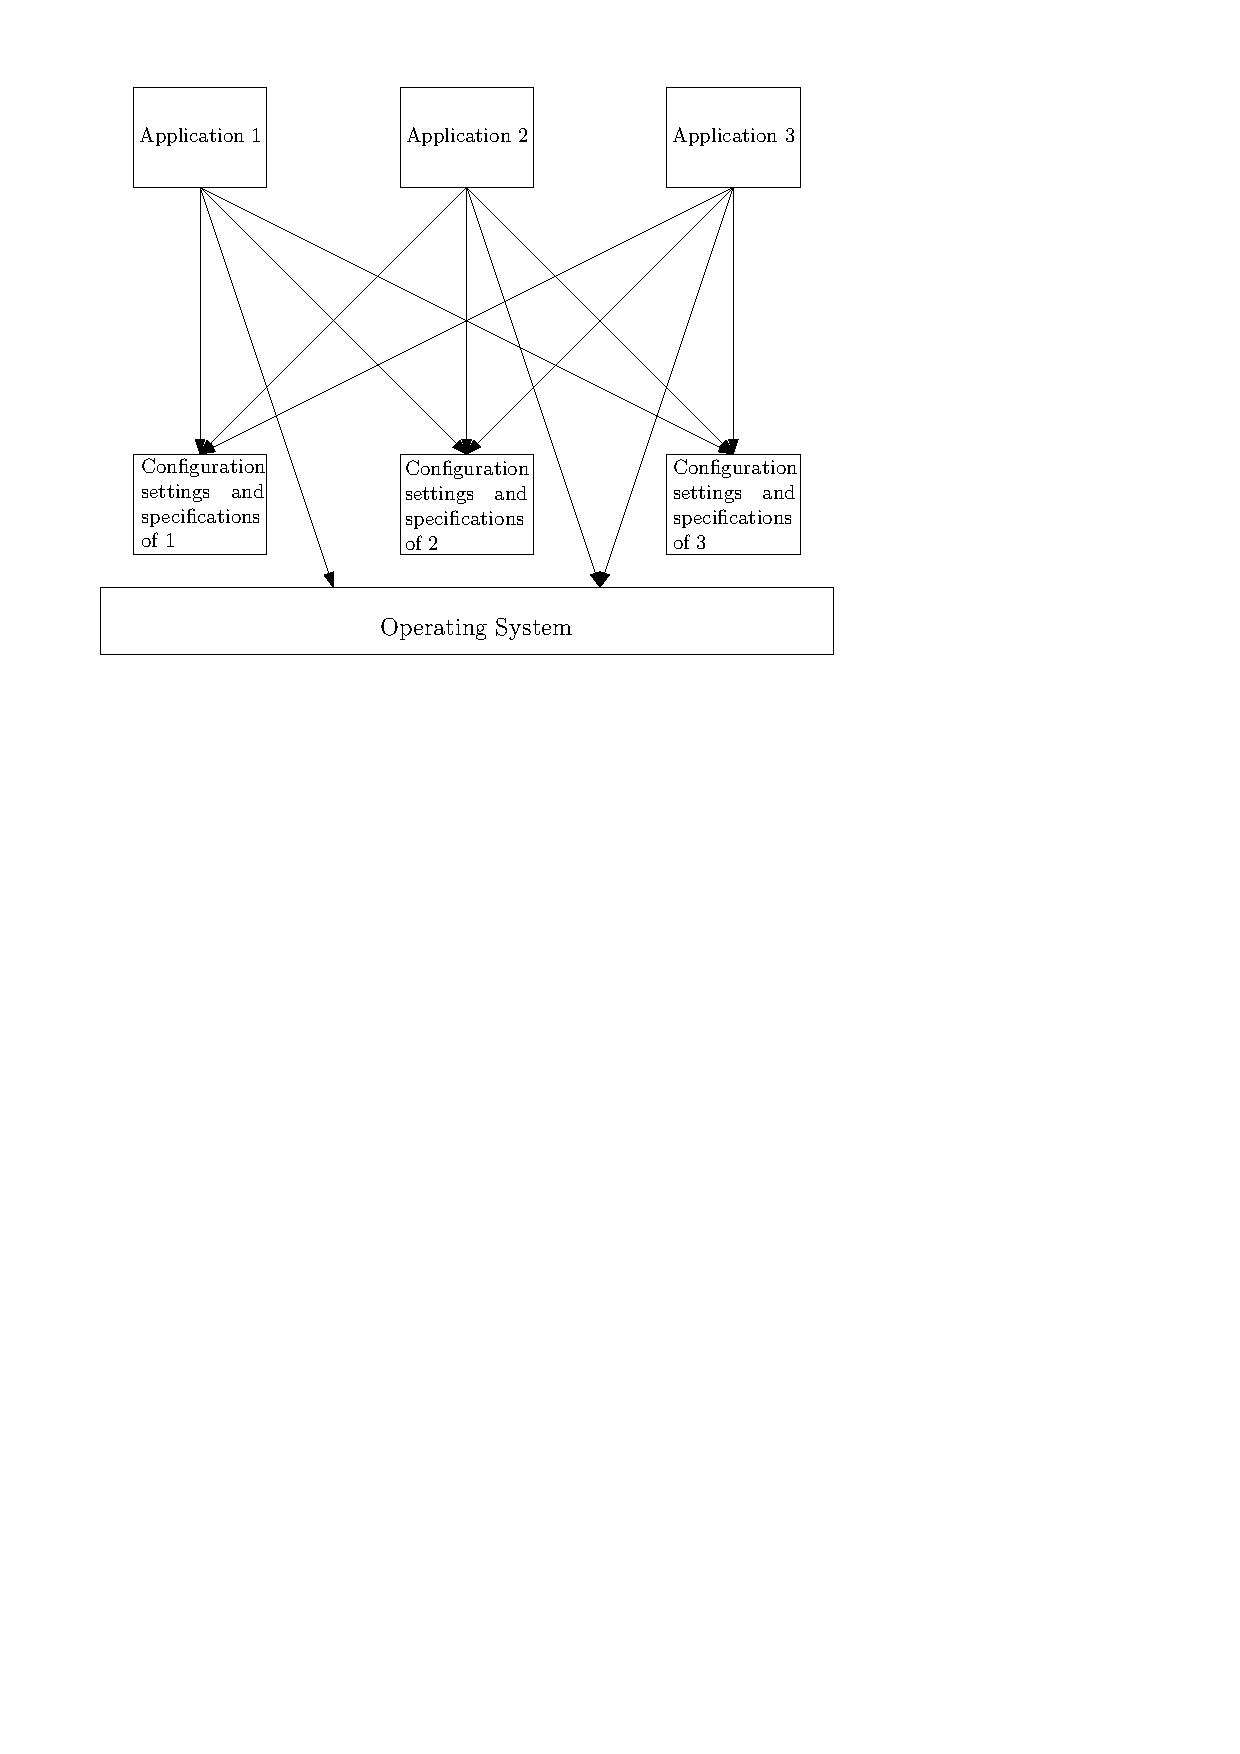
\includegraphics[scale=0.7]{cursituation}
\end{frame}

\begin{frame}
	\frametitle{Wanted Situation}
	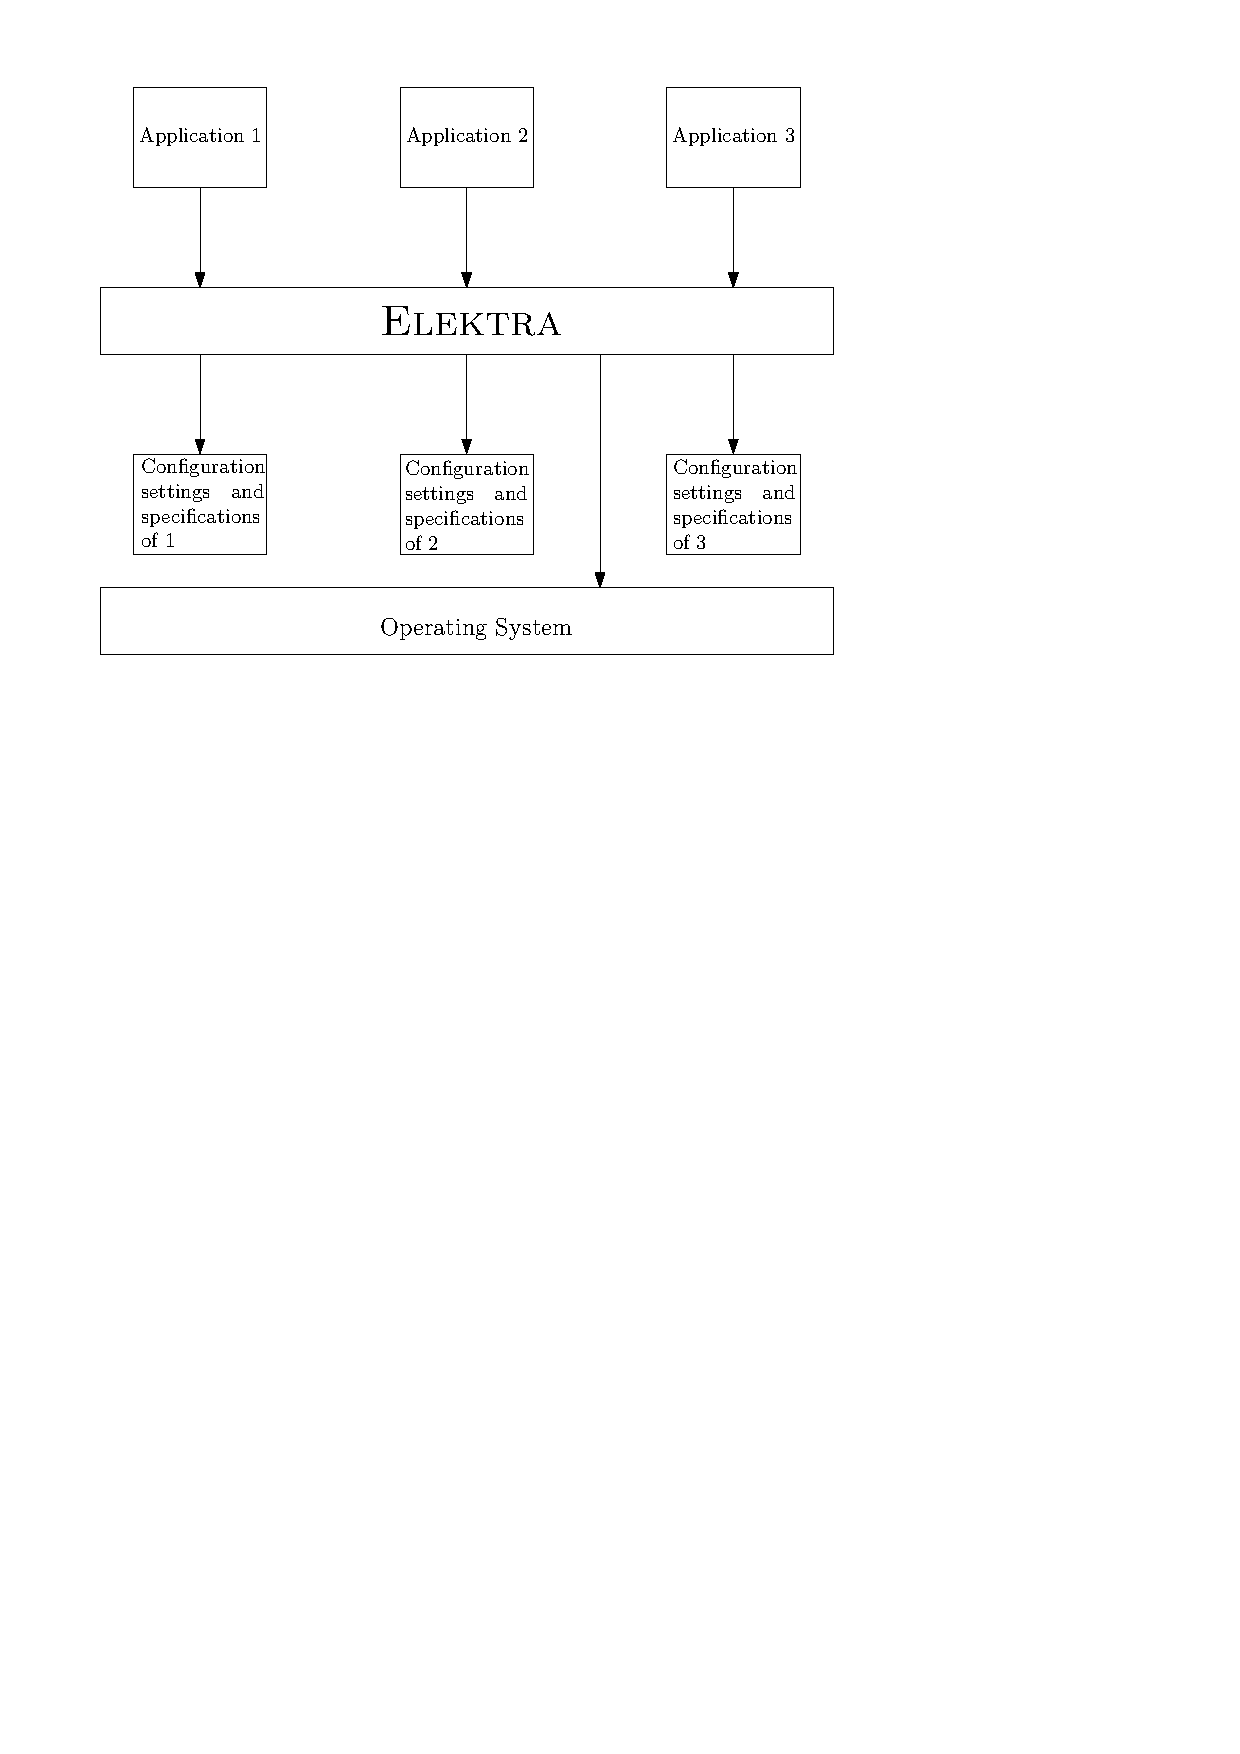
\includegraphics[scale=0.7]{wantsituation}
\end{frame}

\begin{frame}
	\frametitle{Vertical Modularity}
	\begin{alertblock}{Question}
	Explain the content of the figure.
	\end{alertblock}
	\begin{columns}[c]
	\column{7cm}
	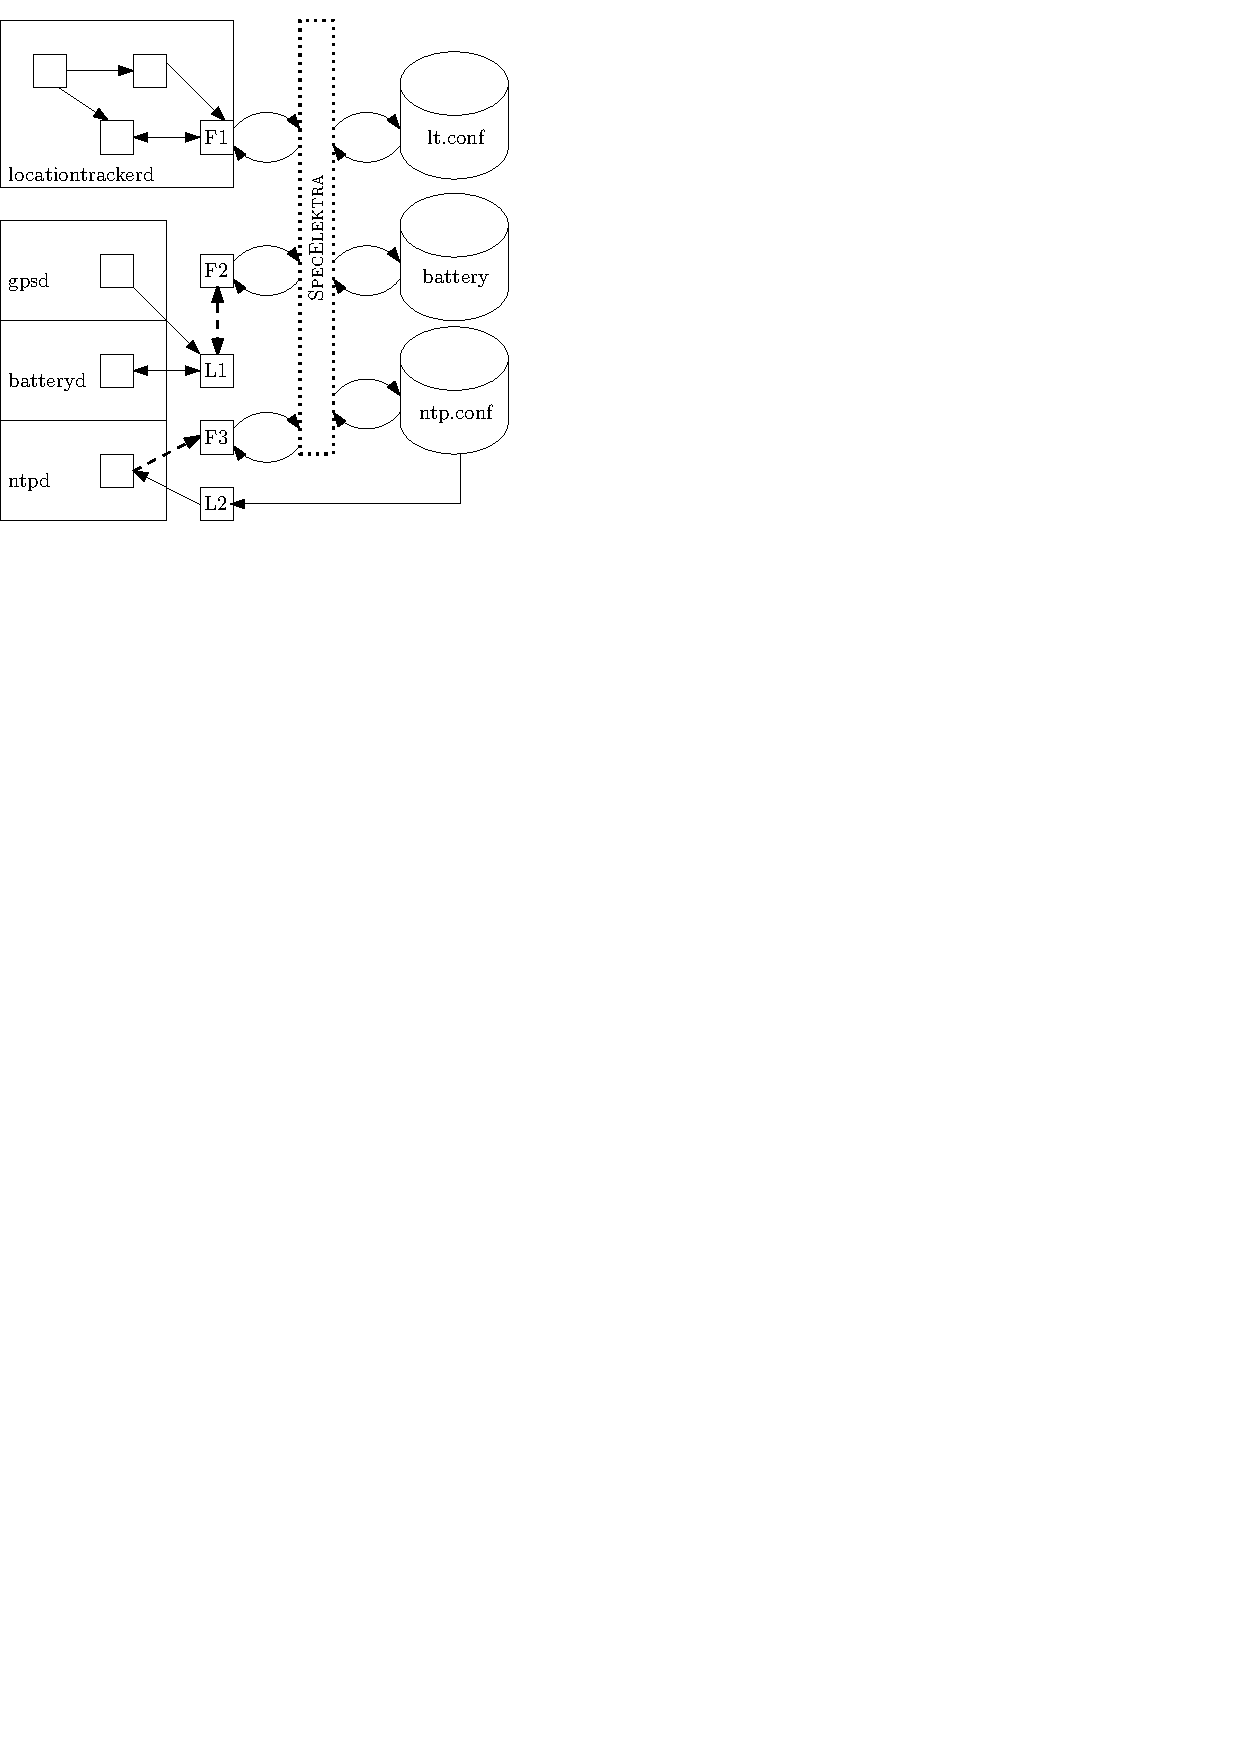
\includegraphics[scale=0.75]{verticalmodularity}
	\column{4cm}<2>
	Needed to keep applications independently.

	Boxes are applications, cylinders are configuration files, F? are frontends or frontend adapters, L? are configuration libraries~\cite{raab2016improving}.
	\end{columns}
\end{frame}

\begin{assignment}
	\begin{task}
	Break.
	\end{task}
\end{assignment}


\begin{frame}
	\frametitle{Metalevels (Recapitulation)}
	\begin{alertblock}{Question}
	Describe the three Metalevels in Elektra.
	\end{alertblock}

	\pause
	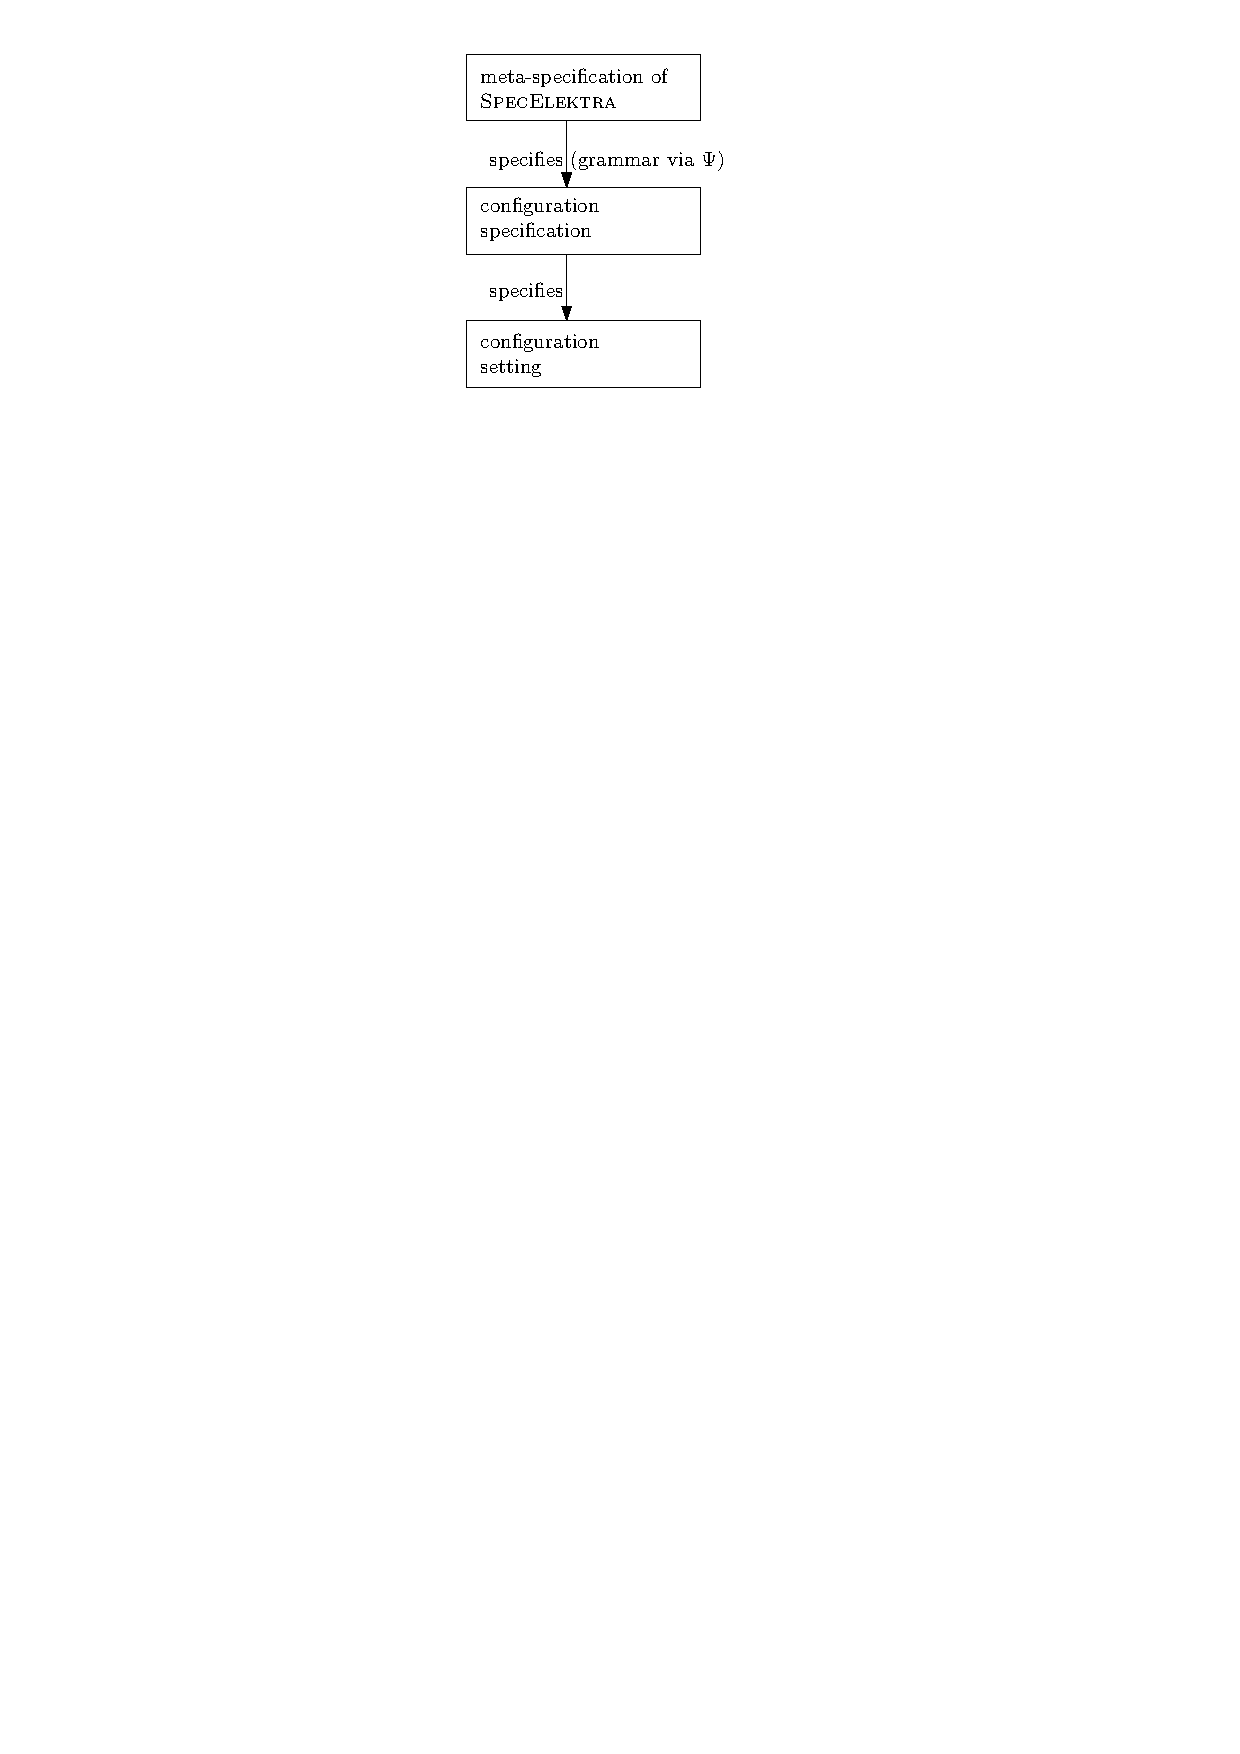
\includegraphics{metalevels}
\end{frame}

\begin{frame}
	\frametitle{Introspection (Recapitulation)}
	\begin{task}
	What is internal and external specification?
	What is introspection?
	\end{task}

	\pause
	\vspace{1em}

	\begin{itemize}
	\item \textit{internal}: within applications' source code
	\item \textit{introspection}: unified get/set access to (meta*)-key/values
	\item access via applications, CLI, GUI, web-UI, ...
	\item access via any programming language (similar to file systems)
	\item GUI, web-UI can semantically interpret metadata
	\item assemble modular parts (validation, logging, \dots)
	\item needed as communication between producers and consumers
	\item essential for \intro[no-futz computing]{no-futz computing}~\citet{holland2001nofutz}
	\end{itemize}
\end{frame}

\begin{frame}
	\frametitle{Introspection vs.\ Code Generation (Recapitulation)}

	\begin{task}
	Advantages/Disadvantages of key database (vs.\ code generation)?
	\end{task}

	\pause

	\setbeamersize{description width=1cm}
	\begin{description}
	\item[$+$] specification can be updated live on the system without recompilation
	\item[$+$] tooling has generic access to all specifications
 	\item[$+$] new features the key database (e.g., better validation) are immediately available consistently
	\item[$-$] more run-time errors due to missing no type safety
	\item[$-$] less techniques for performance improvements
	%\item[$-$] contextual values cannot be used if context differs within same thread
	\end{description}

	\begin{alertblock}{Implication}
	We generally prefer introspection, except for a very thin configuration access API.
	\end{alertblock}
\end{frame}

\begin{assignment}
	\begin{task}
	Break.
	\end{task}
\end{assignment}


\begin{frame}
	\frametitle{Definition Configuration Management (Recapitulation)}

	\begin{task}
	What is Configuration Management?
	\end{task}

	\pause

	\begin{itemize}
	\item is a discipline in which configuration (in the broader sense) is administered.
	\item makes sure computers are assembled from desired parts and the correct applications are installed.
	\item has means to describe the desired configuration of the whole managed system.
	\item ensures that the execution environment of installed applications is as required.
	\end{itemize}
\end{frame}

\begin{frame}
	\frametitle{Possible Benefits of CM (Recapitulation)}

	\begin{task}
	What are the goals of Configuration Management Tools like Ansible?
	\end{task}

	\pause

	\begin{itemize} %[<+-| alert@+>]
	\item The same goals scripts have: \\
		Documentation, Customization, Reproducability
	\item Declarative description of the system \\
		Single Source of Truth 
		(Infrastructure as Code~\cite{waldemar2013testing})
	\item Less configuration drift
	\item Error handling
	\item Pull vs.\ Push
	\item Reusability
	%\item (Resource) Abstractions
	\end{itemize}
\end{frame}

\begin{frame}
	\frametitle{Early detection (Recapitulation)}
	\begin{task}
	When do we want to detect misconfiguration?
	\end{task}

	\pause

	Phases when we can detect misconfigurations:
	\begin{itemize} %[<+-| alert@+>]
	\item Compilation stage in configuration management tool
	\item Writing configuration settings on nodes
	\item Starting applications (load-time)
	\item When configuration setting is actually used (run-time)
	\end{itemize}

	\pause[\thebeamerpauses]

	\begin{alertblock}{Problem}
	Earlier versus more context.
	\end{alertblock}
\end{frame}


\begin{frame}
	\frametitle{Configuration Specification (Recapitulation)}

	\begin{task}
	How can we combine configuration specifications and configuration management?
	\end{task}

	\pause

	\begin{itemize} %[<+-| alert@+>]
	\item configuration settings are simply an instantiation of the configuration specifications.
		Code describing the instantiation is \textbf{CM code}.
	\item configuration design is explicit (like transformations and default values) and can help while writing CM code.
	\item CM code can even be generated from the specification.
	\item access specifications make access trivial via uniform interface.
	\item visibility and similar techniques may help dealing with complexity.
	\end{itemize}
\end{frame}

\begin{assignment}
	\begin{task}
	Break.
	\end{task}
\end{assignment}


\begin{frame}
	\frametitle{Properties (Recapitulation)}

	\begin{task}
	What is idempotent, self-describing, round-tripping configuration?
	\end{task}

	\pause


	\begin{description}[labelsep=3cm,align=right]
	\item[Idempotent]
	yield the same configuration with any number of applications from CM code ($n\ge1$)~\cite{waldemar2013testing}:
	\[
		f(f(x))=f(x)
	\]
	needed to guarantee repeatability

	\item[Self-describing]
	means that from the configuration file alone we are able to derive the correct data structure~\cite{wadler2003xml}.

	\item[Round-tripping]
	means that if a data structure is serialized and then parsed again, we end up with an identical data structure~\cite{wadler2003xml}.
	\end{description}

	The data structure could be a KeySet.
\end{frame}

\begin{frame}
	\frametitle{Popular CMs today}

	\begin{itemize} %[<+-| alert@+>]
	\item CFengine (1993)
	\item LCFG (1994)
	\item Quattor (2005)
	\item Puppet (2005)
	\item Chef (2009)
	\item Salt (2011)
	\item Ansible (2012)
	\item Itamae (2014)
	\item OpsMops (2019)
	\end{itemize}
\end{frame}

\begin{frame}
	\frametitle{Elektra (Recapitulation)}

	\begin{task}
	What is Elektra?
	\end{task}

	\pause

	\begin{itemize}
	\item is not only a key database but a specification language to describe a key database
	\item plugins implement the specification (could be distributed but focus is configuration files)
	\item is library based (no single point of failure, no distributed coordination needed)
	\item supports transactions (persisting whole KeySets at once)
	\item supports integration of existing configuration settings
	\end{itemize}
\end{frame}


\begin{frame}
	\frametitle{Error Messages (Recapitulation)}

	\begin{task}
	What needs to be considered when designing error messages?
	\end{task}

	\pause

	\begin{itemize} %[<+-| alert@+>]
	\item error messages are often the sole data source for admins
	\item configuration design first: avoid errors if possible
	\item error messages should not leak internals~\cite{brown1983error}
	\item ``edit here mentality'': do not point to correct statements~\cite{marceau2011mind}
	\item precisely locate the cause (and do not report aftereffects)
	\item personification~\cite{lee2011personifying}
	\item give context: providing enough information vs.\ not overwhelming the user~\cite{wrenn2017error}

	%mixture from other slides:
	\item pin-point key (which also pin-points to the specification)
	\item let specifications, e.g.\ from validation, override messages
	\end{itemize}
\end{frame}



\begin{assignment}
	\begin{task}
	Break.
	\end{task}
\end{assignment}



\begin{frame}
	\frametitle{Apply to CM (Recapitulation)}

	What can we learn from system administration research?

	\setbeamersize{description width=1cm}
	\begin{description}[<+-| alert@+>]
	\item[$+$] intensive review process catches errors
	\item[$-$] collaboration ineffective
	\item[$-$] context/situational awareness is essential
	\item[$+$] precise editing of configuration files works well
	\item[$+$] self-written tools are very efficient
	\item[$-$] global optimizations difficult
	\end{description}

	\pause[\thebeamerpauses]  %  show after \begin{itemize}[<+->]

	\begin{alertblock}{Idea}
	Replicate parts that work well, automate error-prone parts.
	\end{alertblock}
\end{frame}

%OK
\begin{frame}
	\frametitle{Apply to Elektra (Recapitulation)}

	Elektra's goals are:

	\begin{itemize}[<+-| alert@+>]
	\item being easy to develop new high-level tools
	\item support precise editing:\\ only change the configuration value as specified
	\item provide a common language for both devs and admins
	\end{itemize}

	\pause[\thebeamerpauses]  %  show after \begin{itemize}[<+->]

	Admins/devs still need to:

	\begin{itemize}[<+-| alert@+>]
	\item reduce the configuration complexity
	\item intensively review and improve the specifications
	\item test (and debug) configuration settings
	\end{itemize}
\end{frame}

\begin{assignment}
	\begin{task}
	Break.
	\end{task}
\end{assignment}

\begin{frame}
	\frametitle{Semantics of Configuration Sources}
	\begin{alertblock}{Question}
	What are the semantics of configuration files, environment variables and command-line arguments?
	\end{alertblock}

	\pause
	\begin{itemize}
	\item configuration files: the only one with full IPC capabilities
	\item commandline-arguments:
	\begin{itemize}
	\item passed by main for a new process via \\ (\texttt{int argc, char ** argv})
	\item visible for anyone: \texttt{/proc/self/cmdline}, e.g., via \texttt{ps aux}
%	\item could be passed along to subprocesses but hardly done
	\item need to be parsed by process
	\item portability: differences in parsing
%	\item cannot be changed from outside (requires restart, no IPC)
	\end{itemize}

	\item Environment Variables:
	\begin{itemize}
	\item are per-process
	\item only static view by owner in \texttt{/proc/self/environ}
	\item are not visible from other processes
	\item subprocesses inherit by default
	\item need to be parsed by process (\texttt{[extern] char **environ}) %but API is provided (\texttt{getenv})
%	\item cannot be changed from outside (requires restart or an additional IPC mechanism)
	\end{itemize}
	\end{itemize}
\end{frame}

\section{Conclusion}

\begin{frame}
	\frametitle{Popular Topics 2019S}
	\vspace{-0.55cm}
	\setlength{\columnsep}{-1.3cm}
	\raggedright
	\definecolor{amethyst}{rgb}{0.6, 0.4, 0.8}
	\begin{multicols}{2}
	\begin{description}
	\item[14] {\color{amethyst} tools}
	\item[9] {\color{amethyst} testability}
	\item[9] {\color{amethyst} code-generation}
	\item[7] {\color{amethyst} context-awareness}
	\item[6] {\color{amethyst} specification}
	\item[6] {\color{amethyst} misconfiguration}
	\item[6] {\color{amethyst} complexity reduction}
	\item[5] {\color{amethyst} validation}
	\item[5] {\color{amethyst} points in time} % (early detection)
	\item[5] {\color{amethyst} error messages}
	\item[5] {\color{amethyst} auto-detection}
	\item[4] {\color{amethyst} user interface}
	\item[4] {\color{amethyst} introspection}
	\item[4] {\color{amethyst} design}
	\item[4] {\color{amethyst} cascading}
	\item[4] {\color{amethyst} architecture of access}
	\item[3] {\color{amethyst} configuration sources}
	\item[3] {\color{gray} config-less systems}
	\item[2] {\color{gray} secure conf} %not done
	\item[2] {\color{gray} architectural decisions}
	\item[1] {\color{amethyst} push vs.\ pull}
	\item[1] {\color{amethyst} infrastructure as code}
	\item[1] {\color{amethyst} full vs.\ partial}
	\item[1] {\color{gray} convention over conf} %iguration % not done
	\item[1] {\color{gray} CI/CD} %only uebung
	\item[0] {\color{amethyst} documentation}
	\end{description}
	\end{multicols}
\end{frame}

\begin{frame}
	\frametitle{Wished-For-Topics 2021S}
	\begin{itemize}
	\item Design of Configuration 
	\item Configuration Integration
	\begin{itemize}
	\item Distributed Systems
	\item How to share Configuration between Applications
	\end{itemize}
	\item Configuration Management Tools
	\item Schemata
	\end{itemize}
\end{frame}



\begin{frame}
	\frametitle{Learning Outcomes (TISS)}
	Students will be able to

	\begin{enumerate}
	% Technical and Methodological Knowledge
	\item support configuration management during software engineering,
	\item describe systematic approaches for configuration management and exemplary configuration management tools.
	%Cognitive and Practical Skills
	\item use configuration specification languages,
	\item implement such specified variability during program construction,
	\item apply techniques of quality assurance in configurable applications.
	% Social and Personal Skills
	\item communicate variability with system administrators.
	\end{enumerate}
\end{frame}

\begin{frame}
	\footnotesize
	\frametitle{Learning Outcomes}
	Students will be able to

	\begin{itemize}
	% L01
	\item remember definitions of configuration settings.
	% TODO: meta-levels
	($\rightarrow$ TISS 2)

	% L02
	\item use configuration specification languages.
	(= TISS 3)

	% L03
	\item remember strategies for configuration integration.
	($\rightarrow$ TISS 1)

	% L04
	\item differentiate between configuration sources.
	($\rightarrow$ TISS 1)
	\item unify configuration sources via specifications.
	($\rightarrow$ TISS 1)

	% L05
	%\item {\color{gray} write simple configuration management scripts.}
	\item describe systematic approaches for configuration management and exemplary configuration management tools.
	($=$ TISS 2)

	% L06
	\item {\color{gray} write simple checker plugins.}
	($\rightarrow$ TISS 4)

	% L07
	\item remember terms of properties of CM.
	($\rightarrow$ TISS 2)
	\item remember various strategies for reduction of misconfiguration.
	%\item find unused settings.
	($\rightarrow$ TISS 2)
	($\rightarrow$ TISS 5)

	% L08
	\item recall points of time relevant in configuration management.
	%\item remind some arguments about pull vs.\ push.
	%\item remember various strategies for earlier reduction of misconfiguration.
	($\rightarrow$ TISS 5)

	% L09
	%\item recall a method of avoiding errors.
	\item apply some principles of good error messages.
	($\rightarrow$ TISS 5)
	\item remind some basics of system administrator research.
	($\rightarrow$ TISS 6)

	% L10
	\item design and document configuration settings and specifications.
	($\rightarrow$ TISS 1)
	\item evaluate a configuration system and decide about use of
	($\rightarrow$ TISS 5)
	\begin{itemize}
	\tiny
	\item code generation.
	\item introspection.
	% \item context-awareness.
	\end{itemize}

	% L11
	\item remember connections between the many different topics within CM.
	\end{itemize}
\end{frame}

\begin{frame}
	\frametitle{Map}

	\vspace{-0.5cm}
	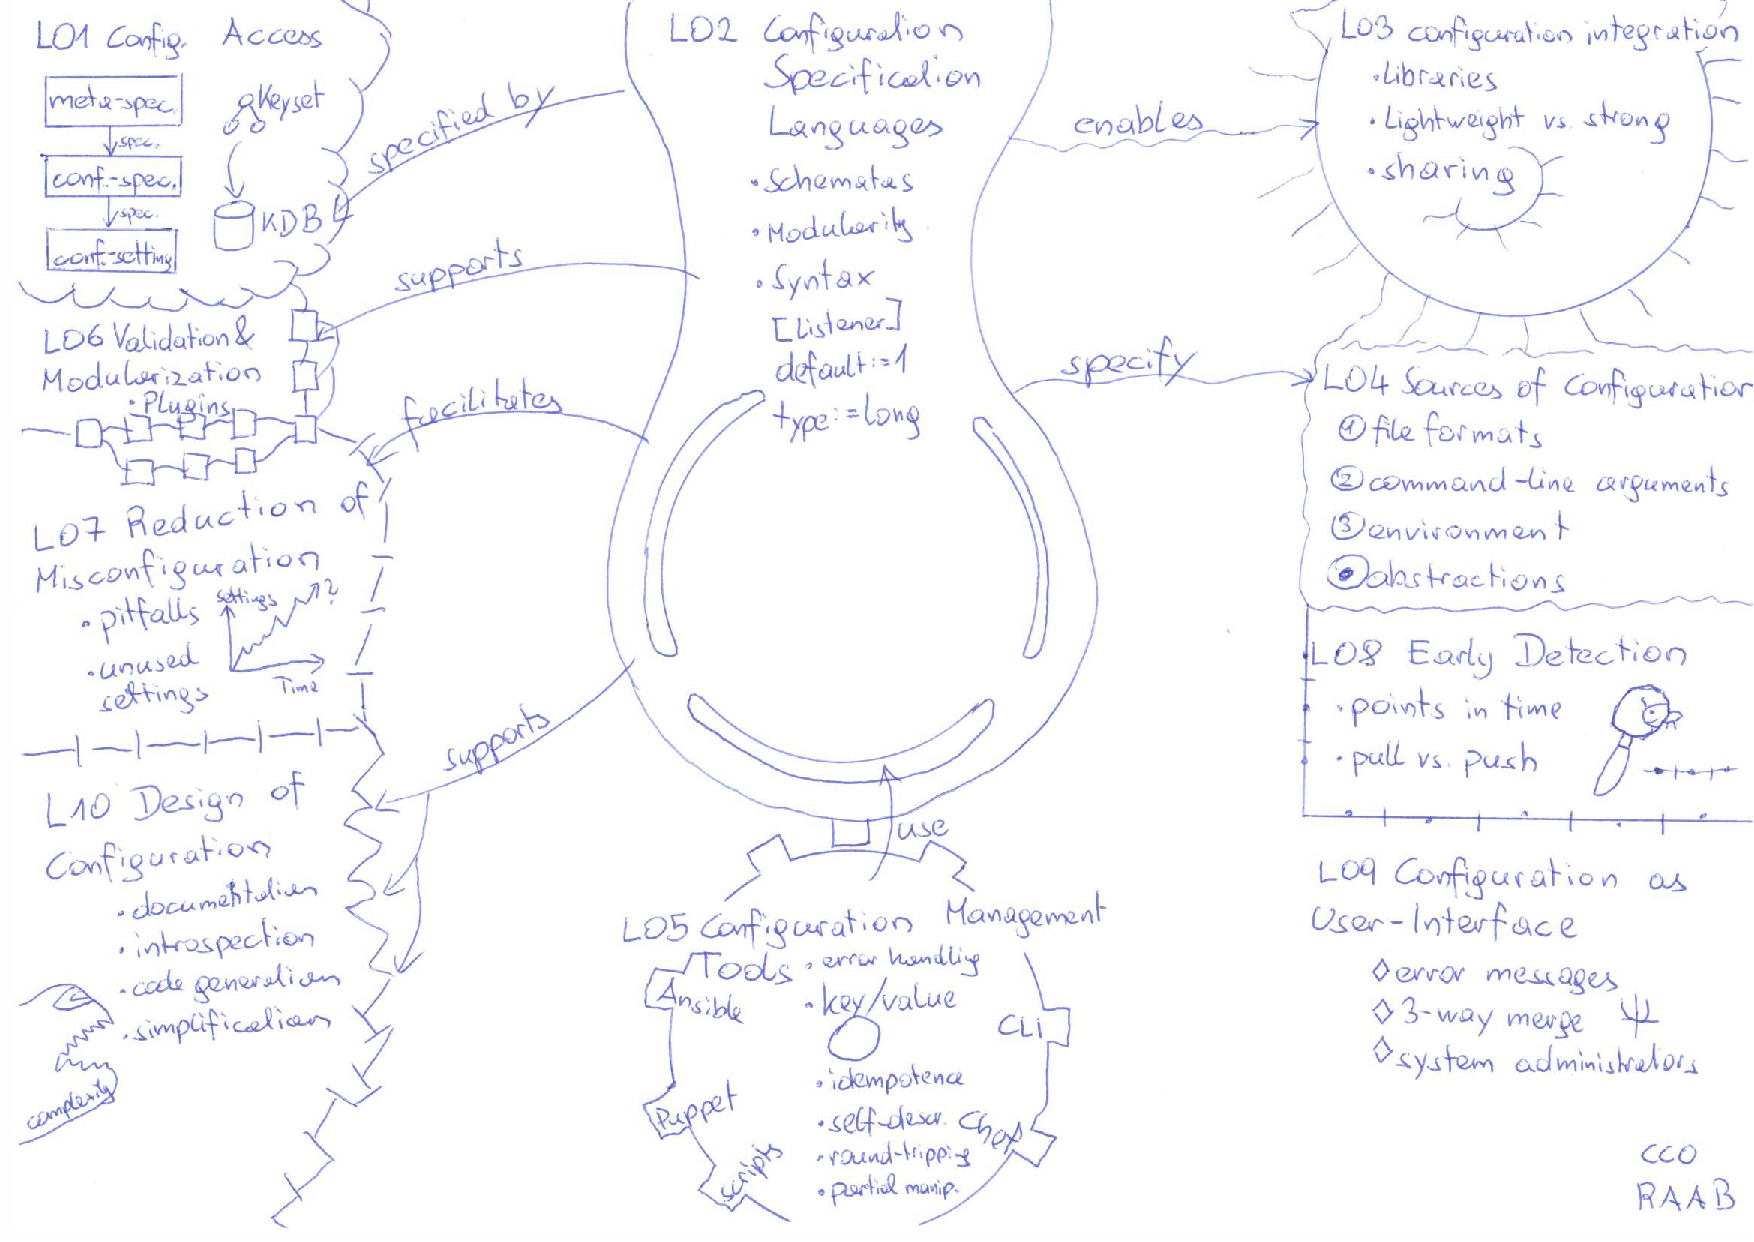
\includegraphics[width=8cm]{pics/map.pdf}
\end{frame}

\begin{assignment}
	\frametitle{Cheat Sheet}
	\begin{task}
	Write your own cheat sheet, maybe similar to map, to be used during exam.
	\end{task}
\end{assignment}

\begin{frame}
	\frametitle{Feedback}
	\hfill \includegraphics[width=2cm]{pics/feedback.png}
	\vspace{-1cm}
	\begin{itemize}
		\item TUWEL Feedback \linebreak
		{\scriptsize \url{https://tuwel.tuwien.ac.at/mod/feedback/view.php?id=1259052}}
		\vspace{0.2cm}
		\item TISS Feedback \linebreak
		{\small from 16.06.2021 00:00 to 14.07.2021 23:59
		\scriptsize \url{https://tiss.tuwien.ac.at/survey/surveyForm.xhtml?courseNumber=194030&semesterCode=2021S}}
	\end{itemize}
\end{frame}

\begin{frame}
	\frametitle{Conclusion}

	Doing CM is easy if the applications support it.
	\vspace{1cm}

	I hope the lecture helped you to know how to write such applications.
\end{frame}




%%%%%%%%%%%%%%%%%%%%%%%%%%%%%%%%%%%%%%%%%% 
\nocite{raab2017introducing}

\appendix

\begin{frame}[allowframebreaks]
	\bibliographystyle{plainnat}
	\bibliography{../shared/elektra.bib}
\end{frame}

\end{document}

